\begin{tikzpicture}[
    font=\footnotesize,
    inputs/.style={rectangle, inner sep=0pt},
    net/.style={draw, rounded corners, very thick, fill=orange!30, inner sep=5pt, font=\footnotesize\sffamily},
    field/.style={inner sep=0pt},
    loss/.style={draw, rounded corners, very thick, fill=red!30, font=\footnotesize\sffamily},
    to/.style={ultra thick, -Triangle},
  ]

  \node[inputs, label=below: Input trajectories] (inputs)
    {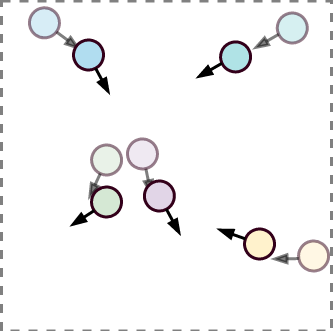
\includegraphics[width=.2\textwidth]{figures/pipeline/input_trajectories.png}};

  \node[field, above=of inputs, yshift=20pt,
    label=above:{Query states}] (query_states)
    {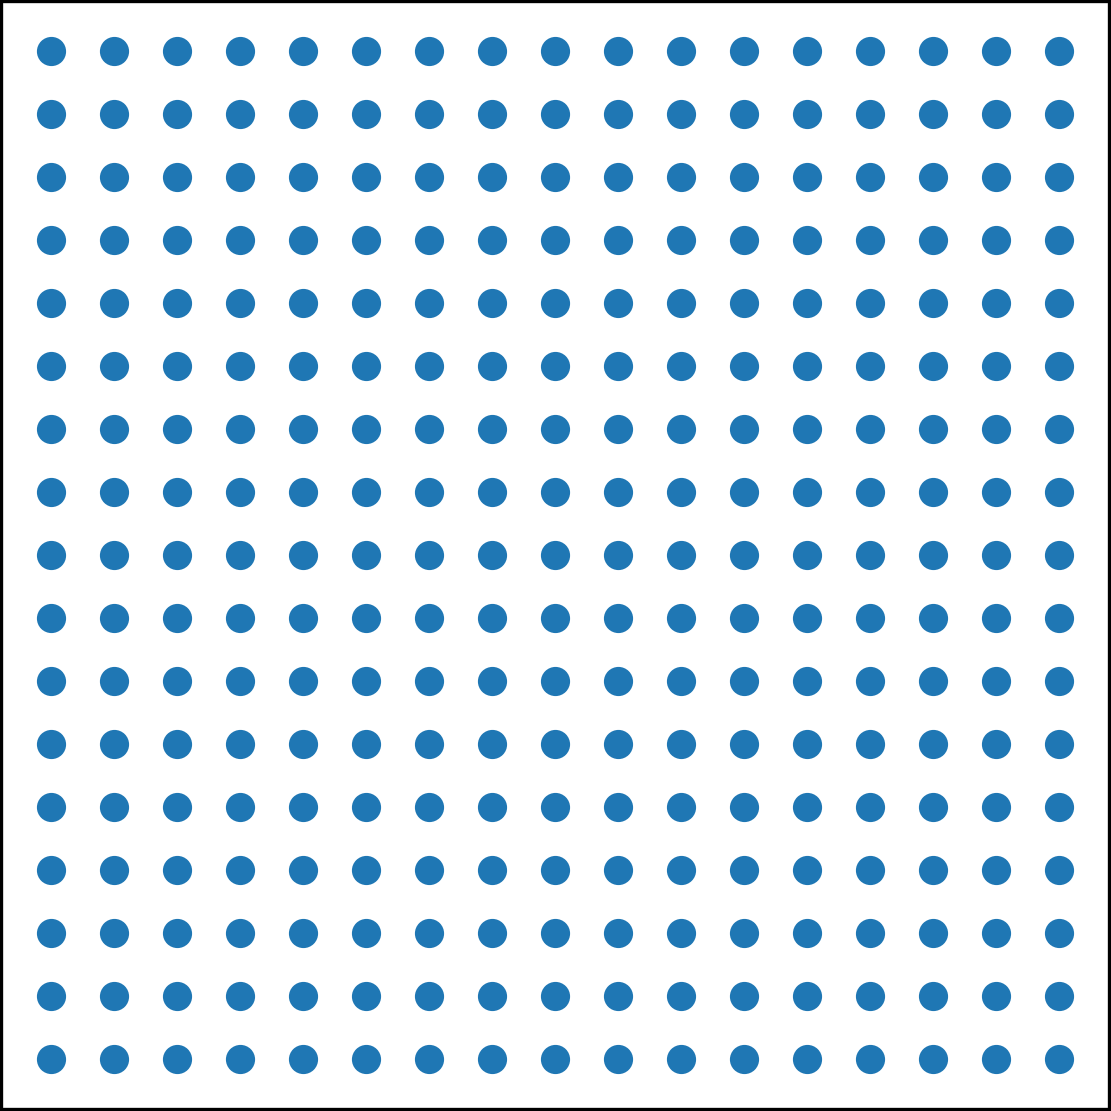
\includegraphics[width=.2\textwidth]{figures/pipeline/8_by_8_meshgrid.png}};

  \node[net, right=of query_states, align=center] (neural_field)
    {Latent\\Neural Field};
  \coordinate (p1) at ($(neural_field.north west)!0.5!(neural_field.west)$);    
  \coordinate (p2) at ($(neural_field.south west)!0.5!(neural_field.west)$);    
  
  \node[field, right=of neural_field,
    label=above:{Predicted field}] (predicted_field)
    {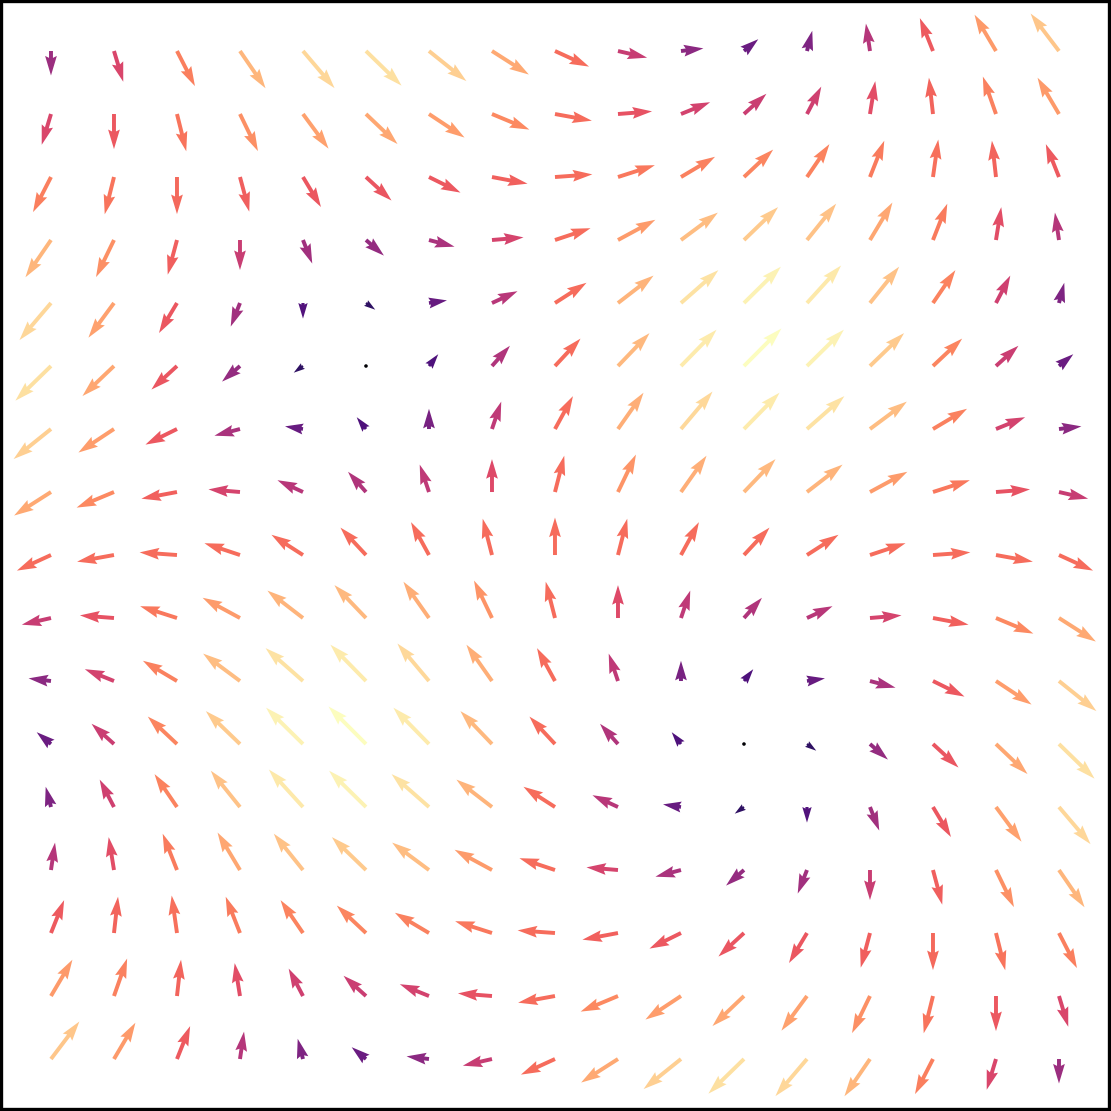
\includegraphics[width=.2\textwidth]{figures/pipeline/8_by_8_meshgrid_inverse_square_law.png}};

  \node[net, align=center] at (inputs-|predicted_field) (gnn)
    {Equivariant Graph\\Neural Network};
   
  \node[inputs, right=of gnn, label=below: Predicted trajectories] (predictions)
    {
\includegraphics[width=.2\textwidth]{figures/pipeline/output_trajectories.png}};
    
  \node[inputs, above=of predictions, yshift=20pt, label=above: Groundtruth trajectories] (gt_trajectories)
    {
\includegraphics[width=.2\textwidth]{figures/pipeline/gt_trajectories.png}};
    
  \node[loss] at ($(predictions.north)!0.5!(gt_trajectories.south)$) (loss)
    {Loss};
    
  \draw[to] (inputs)--(gnn);
  \draw[to] (query_states.east|-p1) -- (p1);
  \draw[to] (neural_field) -- (predicted_field);
  \coordinate (p3) at ($(query_states.east)!0.5!(p2)$);
  \draw[to] (inputs -| p3) |- (p2);
  \draw[to] (gnn)--(predictions);  \draw[to] (predicted_field)--(gnn);
  \draw[to] (predictions)--(loss);
  \draw[to] (gt_trajectories)--(loss);

\end{tikzpicture}
